\chapter{Project Management}


\section{Choice of Process Model}
A strict Scrum based approach to software development was required by the product owner in this project. In addition, the two principles \textit{decide as late as possible} and \textit{deliver as fast as possible}  from  LEAN software development were emphasised by the product owner. The development team had weekly meetings with the product owner and, thus, chose to structure the project in one-week long sprints. 

An agile approach to software development, coupled with short sprints were, in this project, essential to be able to accommodate the product owners focus on the two Lean principles mentioned above. A more traditional plan-based approach would have forced both the customer and the development team to make decisions at a very early stage. 

Much of the communication between the product owner and the development team was based on pitching new ideas and solutions. This process relied heavily on mockups and wireframes, and the agile approach enabled us to easily present solutions at every stage of the development life cycle.


\subsection{Customer Meetings}
Every Thursday, the group met with the product owner for sprint retrospective and planning. During these meetings, the development team began with presenting a demo of the most recent version of the system to the product owner. Based on the feedback of the product owner, we settled on which features to keep, which to discard and which to develop further. This then lead us to the sprint planning of the next sprint, where we decided which features should be included in the next version of the product. 

The customer strongly practiced the Lean principle of \textit{decide as late as possible}, and this was an aspect of the development process unfamiliar to most of the team members. As the development team could not, form the start, neither rely on, nor elicit a fixed list of requirements, these weekly meetings were essential to prevent stagnation of the development. 

\subsection{Supervisor Meetings}
In addition to weekly meetings with the product owner for the development of the solution, the team also had bi-weekly meetings with our course supervisor, NAME, to ensure our progress with the course as a whole. Prior to the meetings we submitted status reports to enable the supervisor to follow our progress and make her aware of any difficulties we might me experiencing. The status report gave a detailed overview of what we had done during the last meeting, what were our plans for the coming sprints, and any difficulties coupled with an updated risk analysis. An example of a status report can be found in Appendix XX, figure XX.


\section{Work Breakdown Structure}

\begin{figure}[h!]
\centering
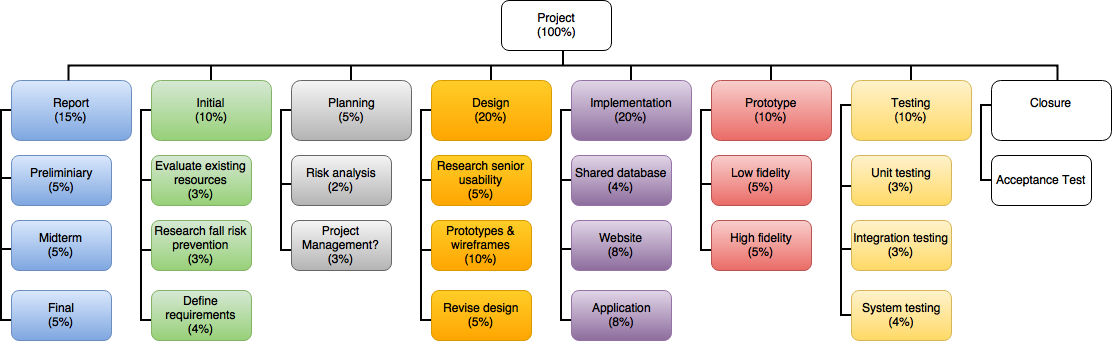
\includegraphics[scale=0.4]{Figures/WBS.png}
\caption{WBS}
\label{fig:WBS}
\end{figure}

\section{Time Constraints}


\section{Risk Analysis}
Managing risk is essential to a software project and a meeting to analyse the risks was settled early. Firstly, in the \textit{risk identification} process, the team identified potential risks and organized them into several larger categories: requirements, team, planning and technical. Secondly, during \textit{risk analysis}, the team estimated both the likelihood and potential impact of each risk. This was done by awarding a number ranging from 1-9 where 1 indicates low likelihood and impact, and 9 indicates high likelihood and impact. Thirdly, the team identified actions to prevent and mitigate the risks during the \textit{risk planning} phase. The outcome of these three first phases is a risk assessment matrix, see appendix A?, Figure \ref{fig:RiskFull}. The matrix lists all the risks accompanied by the likelihood and impact estimates along with preventative and mitigative actions. Below follows a condensed version of the risk assessment matrix, Figure \ref{fig:Risk}, giving a quick overview of how severe the different risks are, with R1, R2, R3, etc referring to Risk 1, Risk 2, Risk 3 and so on. The explanations of each risk can be found in Figure \ref{fig:RiskFull}: 
\begin{figure}[h!]
\centering
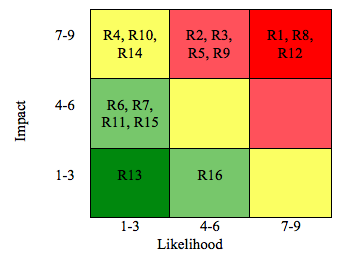
\includegraphics[scale=0.8]{Figures/RiskAnalysis.png}
\caption{Risk Analysis}
\label{fig:Risk}
\medskip
\small
R1, R2, R3, etc refers to Risk 1, Risk 2, Risk 3 and so forth, of the extended risk analysis, see Figure \ref{fig:RiskFull} in the appendix.
\end{figure}

Lastly,  the team decided to perform \textit{risk monitoring} by regularly assessing the risks and revising the risk analysis matrix when needed. 


\section{Project Management Tools}
\subsection{GitHub}
In addition to the source code management provided by git, using gitHub lets us share the repository with all the team members while at the sate time providing several project management features including backlog management, task management, sprint organization and easy communications with the customer. Having code and project management features in the same place eases collaboration as all team members then know where to look for new tasks, and the state of the product. We were not aware of all of these features of gitHub at the beginning of the project and, only towards the end of the project, did the team switch to using gitHub's project management features. 
\subsection{Trello}
Trello is a tool to help people collaborate and organizes your projects into boards. At a glance Trello shows you what is being worked on, who is working on what and what remains to be done. 
As we, as a team,  do not have office space or an alternative fixed location to work from, we do not have a suitable place for a physical Scrum board. Trello is  thus an online alternative to the Scum board which shows the current status fo the project, or at least the sprint.
\subsection{Google Docs}
Google Drive is a file storage and synchronization service that allows users to store files in the cloud, share files, and edit documents, spreadsheets, and presentations with collaborators. It is essential for our team that everyone in the team has the same access to documents relating to the project, and are able to contribute to them.
\section{Group Communication Tools}
\subsection{Slack}
Slack is a cloud-based team collaboration tool used for communication through different chat rooms and channels. We use slack for communication within the team. Slack also has an app which gives you  instant notifications if a group member post anything in one of the channels. Thus, this communication tool is therefore more suitable than for instance email communications as it allows more instant communication. It is also better suited to this project than Facebook, as it allows us to structure our communication into different channels. 

\section{Deviations??}

\section{Team Organization}
\subsection{Responsibilities}
\subsection{Pair-Programming??}

\section{Sprints}
\subsection*{Sprint 1}
\subsection*{Sprint 2}
\subsection*{Sprint 3}
\subsection*{Sprint 4}
\subsection*{Sprint 5}
\subsection*{Sprint 6}
\subsection*{Sprint 7}
\subsection*{Sprint 8}

\section{Gantt Chart}